\chapter{Electrostatic equation -- Capacitance of perforated plate}

\modinfo{Directory}{CapacitanceOfPerforatedPlate}
\modinfo{Solvers}{\Idx{StatElecSolver}}
\modinfo{Tools}{\Idx{ElmerGUI}}
\modinfo{Dimensions}{3D, Steady-state}
\modinfo{Author}{Peter R{\aa}back}


\subsection*{Case definition}

This case presents solving the Poisson equation for electric potential
and calculating appropriate derived quantities, such as
\Idx{capacitance}, based on the result. 
The geometry under study is a perforated plate.

The shape of the holes is assumed to be square with size $3\times 3$~mm$^2$.
The holes cover the other plate uniformly so that the size of each unit cell is 
$10\times 10$~mm$^2$.
The thickness of the plate is assumed to be 
1.5 mm and the distance from the reference plate 1.0 mm. 
The plate may be assumed to be infinitely large. Due to symmetry considerations it suffices to study
only one quarter of a unit cell.

The results may be compared to the ideal plate capacitor without holes. 
For a plane capacitor, the
capacitance is
\begin{equation}
C=\varepsilon_r\varepsilon_0\frac{A}{d},
\end{equation}
where $\varepsilon_r$ is the relative permittivity, $\varepsilon_0$
is the permittivity of vacuum, $A$ is the area of a capacitor plate,
$d$ is the separation of the capacitor plates, and $\Phi$ is the
potential difference between the plates.
For the case under study we get an approximation $C=221.36~fF$.


\subsection*{Preliminaries}

The definitions for the electrostatic equation might not have been loaded into ElmerGUI by default. Check the 
\texttt{Model/Equation} menu
to verify the situation. If electrostatics is not present  
one needs to load definitions for it before starting the simulations.
\ttbegin
File 
  Definitions
    Append -> electrostatics.xml
\ttend
The additional definitions should reside in the directory \texttt{edf-extra} within the distribution.
Moving the desired \texttt{xml} files to the \texttt{edf}-directory enables automatic loading of the 
definitions at start-up. By inspecting the definitions in the \texttt{Elmer Definitions File editor} one
may inspect that the new definitions were really appended. 


\subsection*{Meshing}

In this case meshing is performed using ElmerGrid format in file \texttt{hexhole.grd} and the ElmerGrid plugin within ElmerGUI. 
The default mesh is OK and therefore no modifications are needed by the user. 

Elmer does not operate an any particular units but usually SI-units 
are preferred. We therefore choose to scale the problem with 0.001 so that these measurements will be in mm.  

Load the mesh file.
\ttbegin
File 
  Open -> hexhole.grd
\ttend
You should obtain your mesh and may check that it consists of roughly of 33\,159 nodes and of 
29\,610 linear hexahedral elements.


\begin{figure}[h]
\centering
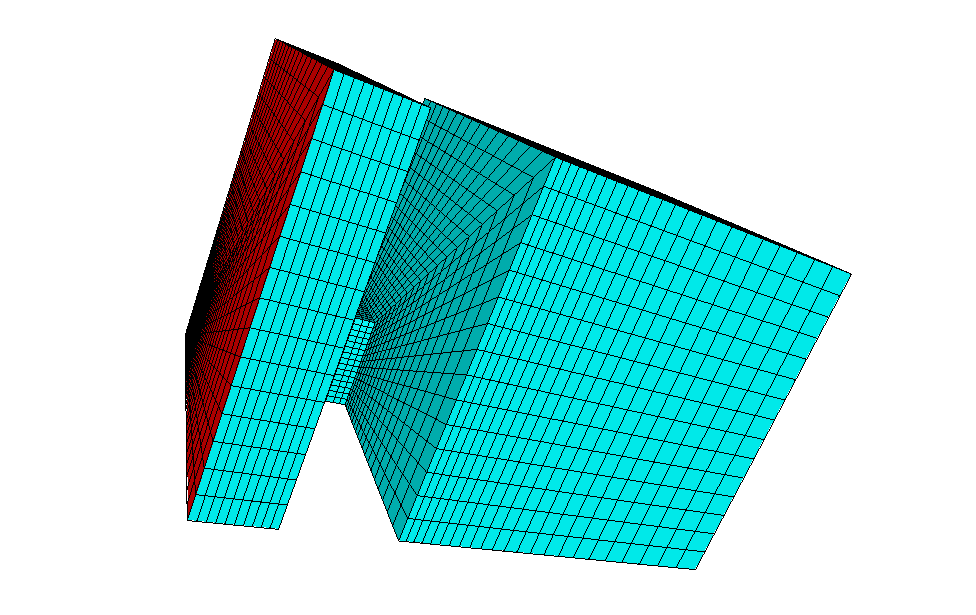
\includegraphics[width=140mm]{HexholeElmerGUI}
\caption{The mesh with one highlighted backplate as seen in ElmerGUI}\label{fg:hexhole_elmergui}
\end{figure}  


\subsection*{Case setup}

After we have the mesh we start to go through the Model menu from the top to bottom. 
In the Setup we choose things related to the whole simulation such as file names, 
time stepping, constants etc.
The steady-state simulation is carried out in 3-dimensional Cartesian
coordinates. We want to work in mm so we need to scale the mesh with a factor 0.001. 
\ttbegin
Model
  Setup 
    Simulation Type = Steady state
    Coordinate Scaling = 0.001
\ttend
In the equation section we choose the relevant equations and parameters related to their solution. 
In this case we'll have only the electrostatics solver. 

When defining Equations and Materials it is possible to assign to the bodies immediately, or to use mouse
selection to assign them later. In this case we have just one body and therefore its easier to assign 
the Equation and Material to it directly.

In the solver specific options we want to activate some flags that are needed to invoke the 
computation of derived fields. 
For the linear system solvers we are happy to use the defaults. One may however, try out different
preconditioners (ILU1,\ldots) or direct Umfpack solver, for example.
\ttbegin
Model
  Equation
    Name: Electrostatics
    Apply to Bodies: 1
    Electrostatics
      Active: on
      Edit Solver Settings
        Solver specific options
          Calculate Electric Field:     True
          Calculate Electric Energy:    True
    Add 
    OK
\ttend        

The Material section includes all the material parameters.
In this case we only have the relative permittivity $\varepsilon_r$ which we could set to one.
Alternatively, we can obtain it automatically by choosing the properties of air. 
\ttbegin
Model
  Material
    Add 
      Material library
        Air (room temperature)
      Apply to bodies: Body 1 
      Add 
      OK
\ttend


We have two boundary conditions for the potential at the ground and at the capacitor. For other boundaries the do-nothing boundary results to zero flux over the boundary.
\ttbegin
Model
  BoundaryCondition
    Name: Ground
    Electrostatics
      Potential: 0.0
    Add
    New

    Name: Capacitor
    Electrostatics
      Potential: 1.0
    Add
\ttend   

The conditions may also be assigned to boundaries in the Boundary condition menu, or 
by clicking with the mouse. Here we use the latter approach as that spares us of the 
need to know the indexes of each boundary.
\ttbegin
Model
  Set boundary properties
    Choose the backplate -> set boundary condition Ground
    Choose the four pieces of the perforated plate -> set boundary condition Capacitor
\ttend

For the execution 
ElmerSolver needs the mesh files and the command file. We have now basically defined
all the information for ElmerGUI to write the command file. After writing it we may also visually 
inspect the command file.
\ttbegin
Sif 
  Generate
  Edit -> look how your command file came out  
\ttend

Before we can execute the solver we should save the files in a directory. The project includes
all the files needed to restart the case.
\ttbegin
File 
  Save Project
\ttend

After we have successfully saved the files we may start the solver
\ttbegin
Run
  Start solver
\ttend
A convergence view automatically pops up showing relative changes of each iteration.
The equation is fully linear and hence only two iterations are needed -- the second 
one just ensures that convergence of the non-linear level was really obtained. 
The norm of the solution should be roughly~0.8846.


\subsection*{Numerical results}

The numerical results obtained for capacitance and electric force are compared
to those of a complete plane capacitor. 

The results of the simulation as well as the comparison to the
complete plane capacitor values are shown in Table~\ref{tab_elstatics}. 

\begin{table}[htb]
\caption{Comparison of numerical results to analytic values}
\label{tab_elstatics}
\begin{center}
\begin{tabular}{lll} \hline
relh & C(fF) & ratio \\ \hline
1.0  & 216.37    & 0.977       \\
0.7  & 216.34    &        \\
0.5  & 216.32    &        \\ \hline
\end{tabular}
\end{center}
\end{table}



\subsection*{Visualization}

When the solution has finished we may start the postprocessor to view some results.
Here we assume that we chose the .vtu format for Paraview as output. The opening of Paraview can be done automatically from the \texttt{ElmerGUI} menu, or alternatively manually from Paraview.
\ttbegin
File 
  Open: case0001.vtu
  Apply 
\ttend

You may now choose the fields to be depicted etc. For more information on the use of of Paraview look at 
the documentation of the software. In figure~\ref{fig:hexhole_pot} some examples of visualizations with Paraview are given. 


\begin{figure}[h]
\centering

\includegraphics[width=70 mm]{HexholePotential}
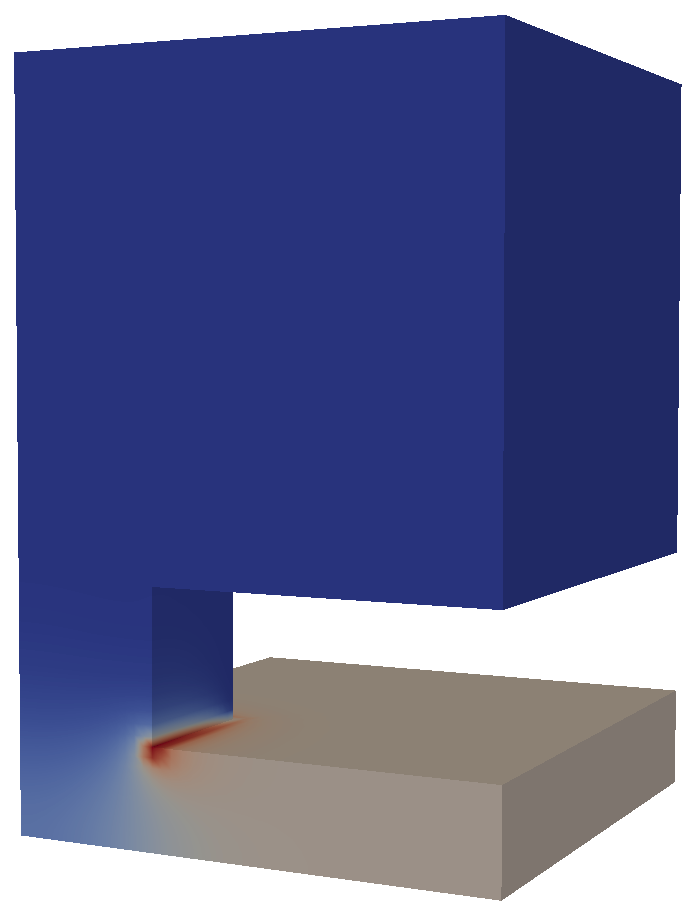
\includegraphics[width=70 mm]{HexholeEnergyDensity}
\caption{The electrostatic potential and the electric energy density of the quarter of  a unit cell of 
a perforated plate capacitor visualized by Paraview.}
\label{fig:hexhole_pot}
\end{figure}  

